
\chapter{Diskussion}

\begin{draft}

I detta kapitel diskuteras projektets genomförande, resultat,
vidareutvecklingsmöjligheter och etiska aspekter.

Till att börja med vill vi säga att hur domänspecifika språk kan kombineras med
fysik inte var något vi visste när projektet startade. En stor del av arbetet i
början av projektet ägnades därför åt att försöka komma på olika sätt att
använda dem ihop med olika fysikaliska områden. Det gjordes många experiment
innan vi hittade sätt att skapa domänspecifika språk till fysik som var annat än
triviala implementationer av formler, till exempel att formlen för
rörelseenergi, $E_k = \frac{mv^2}{2}$, kan skrivas som \texttt{ek m v = m * v *
v / 2} i Haskell. Detta spånande och experimenterande ledde till slut till att
vi kunde se en slags strategi för hur man kan kombinera dem, vilket blev den
metodik som beskrivs i avsnitt~\ref{sec:konstruktion}. Det vi vill poängtera är
med andra ord att det har varit svårt och oklart hur projektet skulle föras
framåt eftersom det inte funnits någon klar och tydlig väg att följa.

\section{Genomförandediskussion}

Under projektets genomförande har det gjorts flera val av teorier och metoder
att använda. Självklart behöver inte dessa val vi gjorde vara de bästa.
Därför kommer vi här kritisera dem och föreslå andra möjliga val. Närmare
bestämt kommer utvärderingen, urvalet och Literate Haskell diskuteras.

Utvärderingen som gjordes under projektet kan kritiseras på flera sätt. För det
första bestod testgruppen av väldigt få personer, enbart tre stycken. Fler
personer hade behövts för att få ett mindre snävt underlag. För det andra hölls
utvärderingen under en ytterst kort tid, ungefär en timme. I början av den
timmen såg de läromaterialet för första gången och resterande tid läste
testgruppen det. Utvärderingen hade behövt vara längre för att låta testgruppen
i lugn och ro arbeta igenom ett par kapitel, inklusive att följa med i
programmeringen som gjordes i läromaterialet. För det tredje var vi inte tydliga
med vad för frågor vi ville ha svar på, utan istället noterade vi testgruppens
spontana reaktioner. Vi ville till exempel veta om de tyckte att domänspecifika
språk gav en rigorös struktur till fysik. Men eftersom vi inte gjorde det
tydligt för testgruppen kunde de heller inte tänka på dessa frågor. Med tanke på
dessa tre brister i utvärderingen är alla slutsatser dragna med utvärderingen
som stöd ytterst osäkra.

Det går även att kritisera hur urvalet av områden gick till under projektet.
Dels kan det ha lett till att inga domänspecifika språk för fysik
implementerades, se diskussionen i avsnitt~\ref{sec:fpf}. Dels skedde urvalet ur
implementatörens perspektiv (det vill säga, vårt) och inte ur användarens
perspektiv (studenten som ska nyttja läromaterialet). Med det menar vi att
områden valdes utifrån hur det implementationsmässigt hängde ihop, till exempel
att matematisk analys är grunden till flera tillämpningar. Istället hade områden
kunnat väljas utifrån de fysikaliska problem studenter ska lösa i Fysik för
ingenjörer, till exempel lutande plan, block och talja eller momentjämvikt, och
utifrån det utforma domänspecifika språk. De olika sätten att tänka vid val av
områden skiljer sig åt och mest fokus under projektet har varit ur
implementationsperspektivet. Visserligen gjordes enstaka försök att tänka på det
andra sättet också, men vi tyckte det var svårt att skapa några domänspecifika
språk på det sättet, se avsnitt~\ref{sec:lampligt}. Vi hade dock kunnat utforska
detta tankesätt grundligare än vad vi gjort, istället för att avfärda det som
ett svårare sätt att gå till väga.

Till sist kan man kritisera den allmänna metoden som valdes för utformningen av
läromaterialet, nämligen att skriva varje kapitel som en lång, sammanhängande,
löpande text. Lärotexten har skrivits som en berättelse om hur ett
domänspecifikt språk kan implementeras eller tillämpas för olika fysikaliska
områden. Nackdelen är att det blir en passiv inlärning. Läsaren visas hur man
kan göra utan att försöka så mycket själv. Visserligen har övningar inkluderats
i läromaterialet, och läsaren uppmuntras programmera koden parallellt, men det
tenderar ändå att riskera bli en passiv inlärning. Valet att använda Literete
Haskell har definitivt bidragit till dessa passiva tendenser. Literate Haskell är
inget annat än en färdig implementation fast mer väldokumenterad och anpassad för
människor än en vanlig programfil. Det kan till och med vara så att Literate
Haskell är sämre än ``bara'' Haskell, med avseende på aktivt lärande, då det är
enklare att ändra och experimentera med en programfil utan prosa i vägen. Under
projektets genomförande hade det därför varit av intresse att undersöka
alternativa sätt att utforma lärotexten som uppmuntrat ett mer aktivt lärande.
Det hade till exempel kunnat vara att presentera iden bakom fysikaliska
dimensioner, och sedan låta studenten själv skapa implementationen. Något enkelt
exempel hade kunnat visats först för att ge någon slags fingervisning om hur man
kan göra.

\section{Resultatdiskussion}\label{sec:res_disk}

Detta kapitel inleds med en övergripande diskussion om det resulterande
läromaterialet, för att sedan övergå till en något mer generell diskussion kring
kombinationen av domänspecifika språk och fysik.

I projektets mål och avgränsningar stod det att vi skulle börja med klassisk
mekanik, för att i mån av tid även behandla termodynamik och våglära. Hur långt
hann vi? I avsnitt~\ref{sec:res_laromaterial} nämns att de tre grundläggande
områdena dimensioner, matematisk analys och vektorer är färdiga, samt de
komposita områdena partikelmekanik, gungbräda och krafter på lådor. Med andra
ord har mekanik påbörjats, men inte termodynamik och våglära. Men hur mycket är
kvar? Det som återstår enligt oss är att tillämpa de grundläggande områdena på
fler fysikaliska problem utöver gungbräda och krafter på lådor. Vi tror att de
tre grundläggande områdena som är färdiga räcker. Förutom fler tillämpningar kan
man utveckla mer fördjupande områden, till exempel bevisföring, något som
nämndes i avsnitt~\ref{sec:res_laromaterial} att det påbörjats. Det är dock värt
att nämna att vi är mycket nöjda med det material som vi har producerat, våra
kapitel är väl avgränsade och är utformade och implementerade på det sätt som vi
tycker att de bör implementeras. 

En annan del av målet var att läromaterialet skulle vara lättillgängligt genom
sitt språkbruk, publicering på en hemsida och fri tillgång till källkoden.
Vi kan genast konstatera att de senare två har genomförts. Vi passar även på att
säga att vi tycker att en lättanvänd hemsida är trevligare att använda än
PDF-filer eftersom de inte har sidbrytningar, fixa sidmarginaler med mera. Detta
är visserligen små detaljer, men tillsammans påverkar de upplevelsen i stort. Vi
tycker även att språket i läromaterialet är någorlunda lättsamt då vi skriver
talspråkligt och vardagligt, och förklarar svårigheterna grundligt. Språket hade
dock kunnat vara ännu mer vänligt. Till exempel framställer vi olika koncept som
``väldigt enkla'' fastän läsaren kanske inte alls tycker det.

Vem är detta läromaterial relevant för? Visserligen är målgruppen datastudenter
men vi tror att det kan vara relevant för fler än så. Framförallt har vi
personligen dragit nytta av det när vi konstruerade det, eftersom det gav oss
fördjupade kunskaper i fysik, domänspecifika språk och Haskell. Läromaterialet
kan även vara intressant för fysiklärare. Fäldt nämnde till exempel att han
tyckte det rigorösa tankesätt läromaterialet skolar in läsaren i kan vara
användbart även i traditionell fysikundervisning. Fysiklärare skulle därför
kunna finna intresse i att undersöka hur ett sådant här läromaterial kan
integreras i undervisningen.

En del av projektets mål var att diskutera kombinationen av
domänspecifika språk och fysik. I de tre följande avsnitten diskuterar vi därför
läromaterialets fokus på matematik och Haskell istället för fysik, vilka
fysikaliska områden som var lämpliga att göra domänspecifika språk till samt om
det finns en pedagogisk nytta i att kombinera de två. Diskussionen är till
största del baserad på våra erfarenheter efter att ha implementerat ett flertal
domänspecifika språk relaterade till fysik, men de är även baserade på
uppfattningar från testgruppen och fysikläraren.


\subsection{Om läromaterialets fokus på matematik och Haskell snarare än
fysik}\label{sec:fpf}

Målet med läromaterialet var att lära ut fysik på ett roligt och lättförståeligt
sätt. Dock syns det i resultatet, avsnitt~\ref{sec:res_laromaterial}, att det
stora fokuset lagts på att förklara och lära ut matematik och Haskell. Varför
blev det så? Vi menar att det finns flera anledningar till detta. 

Problemet med att prata om en egen implementation av fysik är att fysik inte är
ett helt eget område. Det är snarare så att fysik kan ses som tillämpad
matematik, att fysik använder matematiken för att beskriva det fysikaliska
universum vi lever i. Det blir därför naturligt att när den faktiska
implementationen av dessa beskrivningar och lagar sker, så sker de med hjälp av
matematiken. Att ett stort fokus läggs på matematiken är alltså en
konsekvens av fysiken i sig själv. Att fysik är tillämpad matematik illustreras i figur~\ref{fig:xkcd}, som även visar mer generellt hur en kedja av områdena är tillämpningar av varandra.

\begin{figure}[tph]
  \centering
  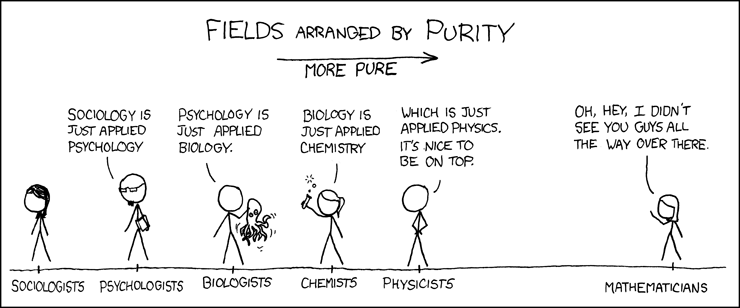
\includegraphics[width=0.9\textwidth]{figure/purity.png}
  \caption{\href{https://xkcd.com/435/}{Purity} av
  \href{https://xkcd.com}{xkcd.com} licensierad under
\href{https://creativecommons.org/licenses/by-nc/2.5/}{CC BY-NC}. Bilden beskriver hur fysik är en tillämpning av matematik. Det är i själva verket
så att en kedja av områden kan betraktas som tillämpningar av
varandra.}\label{fig:xkcd} 
\end{figure}

Självklart ingår det också en stor del problemlösning inom fysik, den faktiska
tillämpningen av de beskrivningar och lagar som matematiken ger oss. Men
problemlösning är något som vi tycker är svårt och problematiskt att modellera
som ett domänspecifikt språk, något som diskuteras djupare i
avsnitt~\ref{sec:lampligt}.

Anledningen till att ett stort fokus läggs på Haskell är att de koncept som används är viktiga för läsaren att förstå. Koncepten är ibland inte kända för en läsare med endast en grundläggande förståelse för Haskell och då måste de förklaras tillräckligt ordentligt för att det ska gå att hänga med. Och
eftersom ett syfte med läromaterialet var väcka intresse hos läsaren med
bakgrund inom Haskell så ville vi lägga fokus på att tydligt visa
parallellerna mellan funktionell programmering, matematik och implementationen
av fysik. 

Vi hävdar alltså att fokuset lagts på mer än bara fysik av två skäl: att fysik är tillämpad matematik och att det är viktigt att förklara de Haskell-koncept som används. Men måste
det vara så? Det kan mycket väl vara så att detta fokusskifte har skett på grund
av hur vi valde att genomföra projektet. I ett tidigt skede valde vi söka efter
områden som vi ansåg vara fristående och väl avgränsade, se avsnitt~\ref{sec:valet},
och implementera dessa var för sig. Utan tvekan har detta sätt att påbörja
projektet påverkat allting som kom därefter. Om vi istället hade utvecklat
läromaterialet som en kombination av olika områden från början hade det kanske
inte varit lika främmande att även baka in problemlösning i detta och på så sätt
fått mer fysik-orienterade domänspecifika språk.

Även tidigare än så går det att vara kritisk till projektets utformning. Varför
valdes Haskell som implementationsspråk? Vi hävdar i teorin~\ref{sec:syntax} att
Haskells typer och fokus på mönstermatchning gör det idealt för implementering
av domänspecifika språk.  Men betyder det att det är idealt för implementering
av fysik? Kanske ett objektorienterat språk som Java hade passat bättre. Att
använda ett språk som inte har en lika stark koppling till ren matematik som
Haskell har hade kanske lett till att det stora fokuset inte låg på matematiken
bakom fysiken, utan istället på fysiken framför matematiken.

\subsection{Vad för slags områden är domänspecifika språk lämpliga att göra
för?}~\label{sec:lampligt}

Under genomförandet av projektet utfördes flera experiment för att bedöma olika
områdens lämplighet för att modelleras med ett domänspecifikt språk. Det visade
sig snabbt att vissa områden lämpade sig mindre väl än andra. Områden
som vektorer och matematisk analys lämpade sig väldigt väl, och ingår även i
läromaterialet (se avsnitt~\ref{sec:res_laromaterial}). Detta var inte särskilt
förvånande eftersom båda områdena är varsin egen gren inom matematiken
och lämpar sig därmed väl för implementering i Haskell som är ett språk med nära
anknytning till matematik. En annan sak som dessa väl lämpade områden hade
gemensamt var en tydlig syntax och en fix struktur som bestod av ``data och
operationer''. Figur~\ref{fig:data_och_ops} visar några exempel på områden med
sina data och operationer.

\begin{figure}[tph]
\centering
\begin{tabular}{l|l}
\toprule
DSL / data & Exempel på operationer \\ \midrule
Dimensioner & Multiplikation, division \\
Vektorer & Addition, skalärprodukt \\
Analys, funktioner & Derivera, multiplicera \\ \bottomrule
\end{tabular}
\caption{Exempeltabell över data och operationer i några domänspecifikaspråk.}\label{fig:data_och_ops} 
\end{figure}

Att notera ur figur~\ref{fig:data_och_ops} är att operationerna inom ett område
görs på en och samma slags data, och sedan resulterar i samma slags data igen.
Det här exemplifieras i matematisk analys, där derivering är en operation, som
görs på en funktion och sedan resulterar i en annan funktion. Detta illustreras
i figur~\ref{fig:analys_op_exempel} där man ser hur derivering av en funktion
resulterar i en ny funktion.

\begin{figure}[tph]
\begin{mdframed}
  \vspace{-0.5cm}
\begin{align*}
  &D : (\R \rightarrow \R) \rightarrow (\R \rightarrow \R) \\
  &D = derivera \\
  &f_1 : \R \rightarrow \R \\
  &f_1(x) = x^2 \\
  &f_2 : \R \rightarrow \R \\
  &f_2(x) = D(f_1) = 2x
\end{align*}
\end{mdframed}
\caption{Ett exempel på hur derivering, en operation i matematisk analys, tar
data av ett slag till data av samma slag igen. I exemplet är $f_1$ och $f_2$
data av slaget funktioner, medan $D$ är operationen derivering. Som synes har
denna operation samma slags data både in och ut.}\label{fig:analys_op_exempel}
\end{figure}

Den fixa strukturen kombinerat med data och operationer gör det enkelt att
modellera dessa områden med datatyper i Haskell. Datatyper har nämligen också en
fix form. Dessutom blir relationen mellan data och operationer i fysik och
datatyper och funktioner i Haskell tydligare, vilket illustreras i
figur~\ref{fig:haskell_fysik_likhet}, som jämför fysikaliska dimensioner med
motsvarande implementation i Haskell. Denna strukturella likhet gör
modellerandet och manipulerandet av data enkel att genomföra rent tekniskt. Men
den innebär också en pedagogisk vinst. Genom att ha strukturerat upp fysik
tydligt i Haskell blir det förhoppningsvis enklare för läsaren att förstå hur
datan hänger ihop rent fysikaliskt. Och även hur relationerna mellan olika
datatyper och funktioner som dyker upp i läromaterialet direkt kan översättas
till motsvarande relationer inom fysik.

\begin{figure}[tph]
  \centering
  \frame{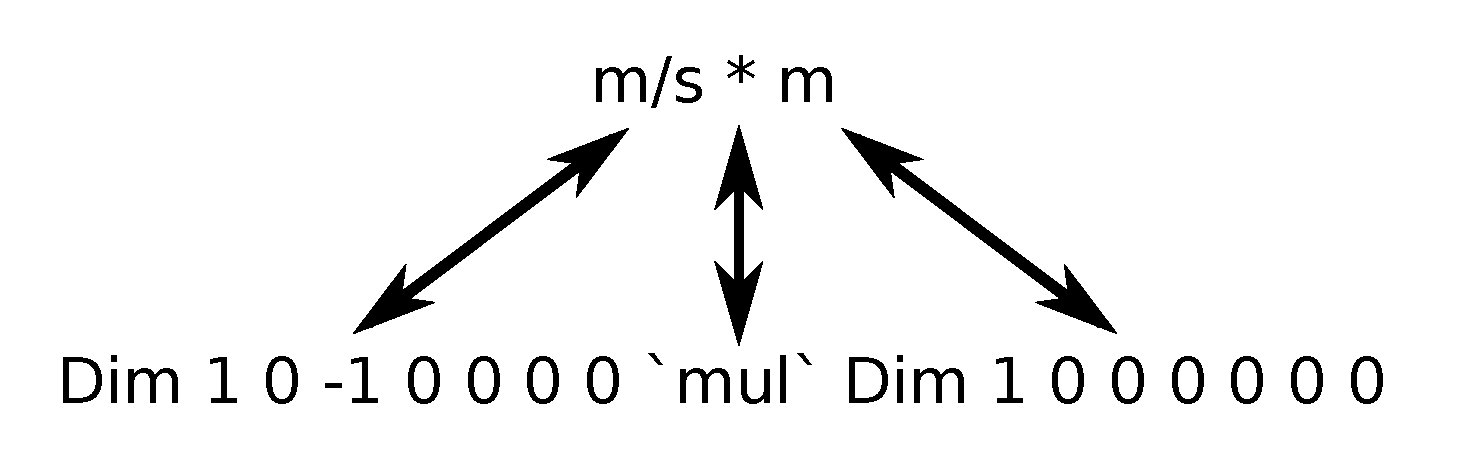
\includegraphics[width=0.6\linewidth]{figure/haskell_fysik_likhet.pdf}}
  \caption{Jämförelse mellan fysikaliska dimensioner (övre raden) och
  motsvarande implementation i Haskell (undre raden). Implementationen kommer
från det resulterande läromaterialet. Mer om implementationen finns att läsa i
avsnitt~\ref{sec:grund_impl}}\label{fig:haskell_fysik_likhet}
\end{figure}

Anledningen till att vi tycker att dessa drag gör ett område mer eller
mindre lämpat för ett domänspecifikt språk kommer från det val vi gjorde tidigt
i projektet, nämligen valet att använda Haskell. I avsnitt~\ref{sec:syntax}
beskriver vi begreppen syntax, semantik och syntaxträd och dess koppling till
både domänspecifika språk och Haskell. Dock finns det ingenting som säger att
man måste lägga ett sådant stort fokus som vi har gjort på till exempel syntaxträd. Hade
vi istället valt bort Haskell till fördel för ett objektorienterat språk hade vår definition av vad som gör ett område lämpat för
implementation helt annorlunda.

I kontrast till dessa lämpliga områden står mindre lämpliga områden (eller
åtminstone områden som vi inte lyckades göra något bra av). Lutande plan är ett exempel på ett mindre lämpligt område. Vad har detta område för drag som gör det mindre
lämpat för ett domänspecifika språk?

När man skapar ett domänspecifikt språk till ett område gör man det genom att
identifiera vad som är syntaxen som används, vad är det för data som modelleras,
vilka operationer som görs på denna data och vad finns det för lagar och samband
som gäller för dessa. Detta sätt att arbeta fungerar bra för områden som är
generella och som går att modellera på ett som tillåter vidareutveckling, såsom
vektorer i flera dimensioner eller vektorer vars komponenter kan vara av vilken
typ som helst.

Ett exempel på ett område som inte har några tydliga data och operationer är just
lutande plan. Ett sådant område har istället teoretiska samband som relaterar
olika egenskaper i systemet till varandra. Ett sådant samband är till exempel $a
= g \cdot \sin(v)$ för det lutande planet i figur~\ref{fig:lutande_plan}.

\begin{figure}[tph]
  \centering
  \frame{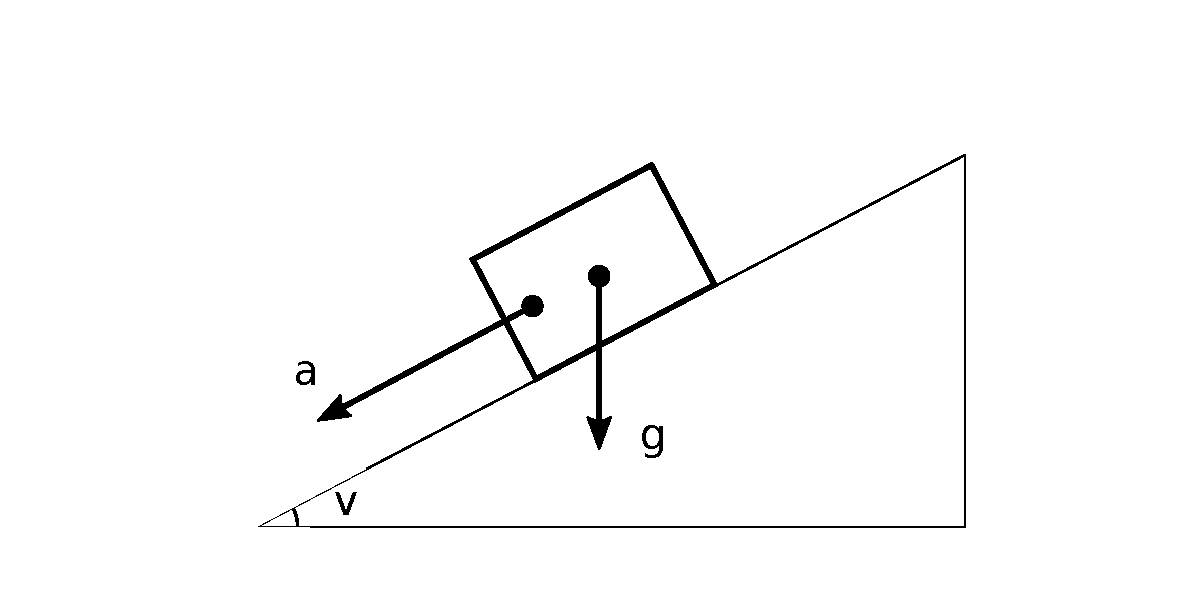
\includegraphics[width=0.5\linewidth]{figure/Lutande_plan.pdf}}
  \caption{Den variant av lutande plan som referas till i exemplet i texten. $a$
  är en lådas acceleration längs med planet, $g$ är tyngdacceleration och $v$ är
  vinkeln. Friktionen antas vara försumbar.}~\label{fig:lutande_plan}
\end{figure}

Samband och ekvationer av detta slag kan visserligen modelleras som ett domänspecifikt
språk, men vi menar att nyttan inte blir stor med det eftersom allt vi då gör är
att skriva de formler som redan finns att tillgå i diverse kursböcker i fysik
utan att tillföra någon ny kunskap och utan att modellera dem på ett generellt
eller unikt sätt. Det man då kan göra är att programmera en ekvationslösare. Men
den hade varit både mekanisk och komplex. Den skulle alltså skilja sig
drastiskt från hur man löser problem för hand och skulle vara svår att förstå.
Alldeles för mycket fokus skulle hamna på algoritmer istället för fysik. Vi
anser även att en ekvationslösare inte hjälper till att lära ut fysik, tvärtom
döljer den matematiken som ligger bakom svaret.

När det kommer till lutande plan och liknande områden är nyckeln att visserligen
känna till vilka samband som gäller, men det är framförallt att veta när man ska
använda dem och hur man tillämpar dem på olika typer av uppgifter. Vi behandlar
därför områden som lutande plan genom att lösa exempeluppgifter modellerade i de
tidigare domänspecifika språk. De tidigare språken tillhandahåller de matematiska
verktyg som behövs för att koda upp lösningar av problem. Därav innehåller det
resulterande läromaterialet, som beskrivs i avsnitt~\ref{sec:res_laromaterial},
inga domänspecifika språk för fysik.

Att vissa områden var mindre lämpliga var ett oväntat resultat i projektets
genomförande. Vid start trodde vi att det skulle gå att göra domänspecifika
språk för alla områden, såväl matematiska som fysikaliska, men som vi här
diskuterat gick inte det. Istället gjordes uppdelningen mellan grundläggande och
komposita områden, som beskrevs i avsnitt~\ref{sec:valet}, så att de fysikaliska
områden (som blev komposita) kunde behandlas som tillämpningar av de
grundläggande områdena.

\subsection{Gör domänspecifika språk att fysik blir mer lättförståeligt eller
intressant?}~\label{sec:bara_fysik}

Är det pedagogiskt att lära ut fysik genom att presentera den med hjälp av
domänspecifika språk? Väcker det intresse för fysik? Tillförde de domänspecifika
språken något i detta läromaterial eller hade det varit bättre att enbart hålla
sig till fysik? Dessa tre frågor diskuteras nedan.

Domänspecifika språk kan betraktas som ``tools for thinking''\footnote{Uttryckt i Patrik Janssons egna ord. Han är föreläsare i DSLsofMath-kursen.}. Med det menas att domänspecifika språk kan användas
till att strukturera ett område så att det blir enklare att få en överblick och
enklare att förstå det. Dimensioner i läromaterialet är ett bra exempel på
detta, se även avsnitt~\ref{sec:grund_impl}. Där konstateras att en godtycklig
dimension kan skrivas som de sju grunddimensionerna med tillhörande exponenter.
Eftersom dimensionerna måste definieras så tydligt att det går att göra ett
program av det tvingas man att ge struktur till dem. Det ger ett nytt,
välstrukturerat och förhoppningsvis enklare sätt att se på dem, vilket vi själva
tycker är meningsfullt.

År 2016 genomfördes ett kandidatarbete på Chalmers liknande
detta~\cite{kandidat2016}. Det kandidatarbetet resulterade också i ett
läromaterial. Skillnaden är att det handlade om signallära medan detta handlar
om fysik. Grundidėn är dock densamma: att använda domänspecifika språk för att
ge struktur till ett annat område.  Detta tycker vi visar att det finns ett
akademiskt intresse för att använda domänspecifika språk i syfte att lära ut,
och att det inte bara är fysik och matematik som är lämpliga områden utan att
den generella idén som vi presenterar i denna rapport även går att applicera på
andra områden. Nyttan med att strukturera upp områden i väl avgränsade och
tydligt definierade delar kanske anses som uppenbar, men frågan om med vilket
verktyg man ska utföra detta är inte lika uppenbar. Vi hävdar att domänspecifika
språk är ett sådant verktyg och att det även är ett mycket bra verktyg att
använda sig av.

En annan aspekt är att när de domänspecifika språken används till fysikalisk
problemlösning är att det måste ske enligt de regler som ställdes upp när de
domänspecifika språken definierades Det går med andra ord inte att fuska och ta
genvägar i beräkningarna. Detta tankesätt tycker Fäldt, se
avsnitt~\ref{sec:res_ake}, är en mycket bra aspekt som förmedlas med att
presentera fysik på detta sätt. Studenten skolas in i att tänka i rigorösa och
kompletta banor.

Det som talar emot
domänspecifika språk när det kommer till fysik är den stora del av problemlösning
som ingår i fysik. Det har att göra med deras olika natur. Domänspecifika språk
har en entydig och fyrkantig struktur medan problemlösning handlar om
kreativitet och nytänkande. Eftersom en stor del i fysik är just problemlösning
kan denna del inte fångas upp med domänspecifika språk. Det skulle till och med
kunna vara en nackdel att kombinera domänspecifika språk och fysik om det leder
till att man tänker alltför fyrkantigt kring fysik. Vi anser dock att
domänspecifika språk har ett värde ihop med fysik just för dessa strukturgivande
möjligheter, även om inte alla aspekter av fysik kan täckas. 

Man kan också
tänka sig att det finns ett värde i ett fånga upp den kreativa problemlösningen
med ett fyrkantigt system och på så sätt stoppa problemlösaren från att göra
misstag. På ett förenklat sätt kan man säga att så länge typsystemet inte klagar
betyder det att man löser problemet på ett korrekt sätt. Igen handlar det om att se
domänspecifika språk som ``tools for thinking'' och inte att vårt
läromaterial kommer att ge alla svaren när det kommer till fysikalisk
problemlösning. Men vad det kan tillföra är en struktur som kan hjälpa
läsaren att enklare komma fram till lösningen, och som garanterar att inga
syntaktiska misstag gjorts.

Hittills har domänspecifika språk framförts som ett sätt att strukturera fysik.
Projektets läromaterial är ett exempel på ett sådant försök. Men läromaterialet
har även haft två andra drag, förutom domänspecifika språk, som skiljer sig från
traditionell fysikundervisning, nämligen ett lättillgängligt språk och en
nogrann genomgång av koncepten. Hade inte detta räckt? Hade fysiken i sig inte
kunnat förklarats bättre om den haft allt fokus?

Vi tror att svaret på båda dessa frågor är ja, med vissa reservationer. Ett
läromaterial om renodlad fysik med ett lättsamt språk och nogrann förklaring av
koncepten hade säkert varit uppskattat. Khan Academy är ett sådant
exempel och som är mycket uppskattat~\cite{khan}. En annan fördel hade varit att en större målgrupp kan nås.
Men då missar man de saker domänspecifika språk bidrar med, nämligen det som
diskuterats ovan: att ge struktur och att lära ut ett rigoröst tankesätt. Man
missar också den \textit{intresseväckande} potentialen.

Domänspecifika språk kan ses som ett sätt göra fysik intressantare. Tycker man
att domänspecifika språk är roligt men inte fysik skulle en överbryggning av dem
kunna leda till att man tycker fysik blir roligare. Detta genom att man ser
parallellerna mellan domänspecifika språk och fysik. Ett exempel är typsystemet i
Haskell och dimensioner i fysik. I bägge världarna får inte olika typer
respektive dimensioner adderas, och vid operationer behandlas de på liknande
sätt. Denna likhet påvisades i läromaterialet genom att implementera fysikaliska
dimensioner i Haskells typsystem, se avsnitt~\ref{sec:res_laromaterial}. Denna
tanke stöds av att även testgruppen tyckte läromaterialet var ett intressant sätt
att presentera fysik på och att vi var inne på rätt spår i vår utformning av
läromaterialet, se avsnitt~\ref{sec:res_test}. Eftersom utvärderingen med
testgruppen var väldigt kort är det dock svårt att dra några säkra slutsatser
med hjälp av utvärderingen. Nyttan med ett större intresse för fysik är att man
då förhoppningsvis är mer motiverad att lära sig fysik för att klara fysikkurser
i skolan. 

Avslutningsvis när det kommer till domänspecifika språks vara eller icke-vara
ihop med fysikundervisning anser vi att en antingen-eller syn inte är bra.
Istället kan man kombinera dem på ett balanserat sätt. Det kan handla om att ha
vissa inslag av domänspecifika språk i en annars traditionell fysikundervisning,
och på så sätt fånga upp de delar domänspecifika språk gör bra i fysik:
strukturera, uppmuntra rigorös problemlösning och väcka intresse. Men samtidigt
förlita sig på traditionella metoder till stor del i bland annat problemlösning
och inte låta fokuset glida för långt från fysik till domänspecifika språk.

\section{Vidareutvecklingsmöjligheter och behov av ytterligare kunskap}

Läromaterialet innehåller domänspecifika språk för de \textit{matematiska}
områdena analys och vektorer. Dessa områden används sedan för att koda upp och
lösa uppgifter av mer \textit{fysikaliska} slag, till exempel lutande plan. Med
andra ord görs inga domänspecifika språk för fysik i sig. En vidareutveckling
hade därmed varit att göra precis det, att inte bara tillämpa matematiska
domänspecifika språk utan göra fysikaliska domänspecifika språk. Det kan vara
saker som ett syntaxträd för ett lutande plans komponenter. Det kan vara ett
syntaxträd för vilka krafter som verkar på fysikaliska kroppar i mekanikproblem.
Det kan till och med vara ett domänspecifikt språk för något så abstrakt som
fysikalisk problemlösning i allmänhet. Vi vet inte hur ett domänspecifikt språk
av detta slag kan se ut, vilket är anledningen till att vi gick den andra vägen,
som vi diskuterade i avsnitt~\ref{sec:fpf}. Att ger mer fysik-orienterade
domänspecifika språk hade därför varit en möjligt vidareutveckling.

En annan möjlig vidareutveckling är att göra en rigorös studie kring de
pedagogiska aspekterna kring kombinationen av fysik och domänspecifika språk.
Detta projekt innehöll enbart en mindre sådan studie. Det som kan vara
intressant att undersöka är om studenter tycker att fysik blir intressantare
genom en kombination av detta slag och kanske därför studerar mer i fysikkursen.
Det hade också varit intressant att undersöka om det rigorösa tankesätt
domänspecifika språk förmedlar, se avsnitt~\ref{sec:bara_fysik}, spiller över och
gör nytta inom traditionell fysikundervisning. Det är inom dessa två frågor det
främsta behovet av ytterligare kunskaper ligger. Målet med ett arbete av detta
slag är trots allt att förbättra fysikkunskaper (genom ökat intresse eller mer
rigorösitet) och då är det av yttersta vikt att undersöka om det faktiskt blir
så i praktiken.

Även det befintliga läromaterialet kan byggas vidare på. I sin nuvarande
form behandlas varken termodynamik eller vågrörelselära något alls. Dessutom lär
det finnas aspekter inom den klassiska mekaniken som fattas.

Slutligen finns det en mycket intressant vidareutveckling som inte alls har
behandlats i detta projekt, nämligen att använda matematiska och fysikaliska domänspecifika språk som
ett syntaktiskt lager mellan användare och en underliggande komplex kodbas. I
många fall kan dessa kodbaser vara implementerade på ointuitivt sätt och utan
någon typsäkerhet. I dessa fall kan det vara mycket användbart med ett
domänspecifikt språk med hög typsäkerhet som möjliggör för användaren att
endast skriva korrekta uttryck och som döljer den bakomliggande komplexiteten. Tänk till exempel på kod i Matlab. Där är det lätt hänt att missa någon detalj i sin implementation så att beräkningarna blir fel. Om ett syntaktiskt lager funnits som krävde att de fysikaliska dimensionerna stämde överens hade vissa misstag kunnat upptäckas vid kompileringstid istället för att kanske inte upptäckas alls. Denna idé framfördes till oss av Jeff Chen\footnote{Jeffs sida på Chalmers:
\url{https://www.chalmers.se/en/education/next-stop/stuamb/Pages/Previous\%20student\%20ambassadors/Jeff.aspx}.}
på Chalmers, men är även någonting som har genomförts på andra områden, till
exempel inom molekylär dynamik~\cite{MD}.

\section{Etiska aspekter}

En bakomliggande tanke vi haft genom hela projektet är att läromaterialet ska
vara fritt tillgängligt för alla, därför har vi valt att publicera det på en
hemsida.  Denna hemsida använder grundläggande HTML och CSS samt javascript.
Javascript är dock inget strikt krav för funktionaliteten. Eftersom hemsidan är
lättviktig bör den fungera väl även på gamla datorer och telefoner, till
skillnad från tunga PDF-filer och många moderna hemsidor. Läromaterialet blir på
detta sätt tillgängligt även för studenter i länder med sämre
internetuppkoppling.

Tanken om tillgänglighet ligger även bakom valet att låta källkoden vara fritt
tillgänglig. Visserligen \textit{är} läromaterialet i princip hela källkoden, det vill säga
har man läromaterialet har man källkoden. Men att ha tillgång till källkoden
direkt har dock fördelar som att man kan följa med i versionshistoriken, man kan
se kommentarer och alternativa implementationer som inte syns i den slutgiltiga
produkten samt att det blir enklare att modifiera källkoden och lära sig om
hemsidans uppbyggnad.  Det handlar om att visa att man är positiv till att andra
tittar hur man gjort och låta andra bygga vidare på ens skapelser. Genom att
sluta oss till skaran som skapar öppen källkod hoppas vi att fler inom samhället
i stort ska gå över till denna modell.

Valet att skriva på engelska har också att göra med tillgängligheten. Fler kan
engelska än svenska. På detta sätt kan läromaterialet komma fler till gagn.

Angående beskrivningen under teori att upplevelsen av materialet är ämnad att
vara rolig, så är det mer tillgängligt för elever som kanske inte hade orkat
läsa en akademisk lärobok. Även om kvalitén i en akademisk lärobok kan vara hög,
är det inte alltid kvalitén kommer till nytta om eleven lägger boken åt sidan på
grund av en impuls att göra något som kan vara mer stimulerande.  Genom att
använda ett enkelt språk, roliga formuleringar och bilder, minskar chansen för
flyktförsök. Detta kan tänkas vara extra viktigt för yngre elever vars kontroll
av uppmärksamhet inte är lika utvecklat som hos äldre men som ändå är
intresserade av fysik på en mer avancerad nivå än de studerar i sin ordinarie
undervisning.

\end{draft}
